\section{February 05}
Today, we will discuss the wave speed in a linear medium. To begin, recall from the first lecture that in a
material, Maxwell's equations read as follows:
\begin{align*}
	\div \mathbf{D} &= \rho_f & \curl \mathbf{E} &= -\partial_t \mathbf{B}\\
	\div \mathbf{B} &= 0 & \curl \mathbf{H} &= \mathbf{J}_f + \partial_t \mathbf{D} 
\end{align*}
Now, we will consider the special case where we have a medium where there are no free charges, no free
currents, and the medium is linear. The first two conditions implies that \( \rho_f \) and \( \mathbf{J}_f\)
are zero, and the last condition implies that \( \mathbf{D} = \epsilon \mathbf{E} \) and \( \mathbf{B} = \mu
\mathbf{H}\). Here, \( \epsilon \) and \( \mu \) are constants. So, Maxwell's equations now read:
\begin{align*}
	\epsilon (\div \mathbf{E}) &= 0 & \curl \mathbf{E} &= -\partial_t \mathbf{B}\\
	\div \mathbf{B} &= 0 & \frac{1}{\mu}(\curl \mathbf{B}) &= \epsilon \partial_t \mathbf{E}
\end{align*}
Notice, these four equations look \textit{exactly} the same as Maxwell's equations in a vacuum, except now
we've replaced \( \epsilon_0, \mu_0 \) with \( \epsilon, \mu \). So, this means that in linear media, \(
\mathbf{E} \) and \( \mathbf{B} \) are still expected to satisfy the wave equation:
\begin{align*}
	(\nabla^2 - \mu \epsilon \partial_t^2)\mathbf{E} &= 0\\
	(\nabla^2 - \mu \epsilon \partial_t^2) \mathbf{B} &= 0 
\end{align*}
These waves propagate with speed \( v = \frac{1}{\sqrt{\mu \epsilon}} \). It should make sense that these two
quantities parametrize the wave speed, since they tell us how easy it is to polarize and magnetize the
material, so in a sense it tells us how easy it is for light to "move through" the material. But, how do we
provably show that increasing \( \mu \) or \( \epsilon \), then the wave speed decreases? To see why, let's
consider our travelling wave as a result of "dipole radiation". 

\subsection{Dipole Radiation}
Consider a bulb, which emits a sinusoidal electric field \( \mathbf{E}_\text{primary} \), that now encounters
a plane made of a different medium (glass, water, etc.). The \( \mathbf{E} \) field emitted by the bulb will
now oscillate the charges in the glass, according to \( x(t) = x_0 \cos( \omega t) \). The electric dipole
moment, is given by \( p(t) = qx(t) = qx_0 \cos (\omega t) \). Based on this motion, the electric field
generated is given by
\[
	\mathbf{E} = \frac{1}{4 \pi \epsilon_0 c^2}\frac{\sin \theta}{r} q \omega^2 x_0 \cos\left[ \omega\left(t -
	\frac{r}{c}\right) \right] \hat{\boldsymbol{\theta}}
\]
The details for why this is will come in when we cover chapter 11. For now, notice that here the \(
\mathbf{E} \) field drops off with \( \frac{1}{r} \) rather than \( \frac{1}{r^2} \) like a point charge.
Now, what is the field created by the entire slab? Let's consider the geometry of the slab as follows:

\begin{center}
	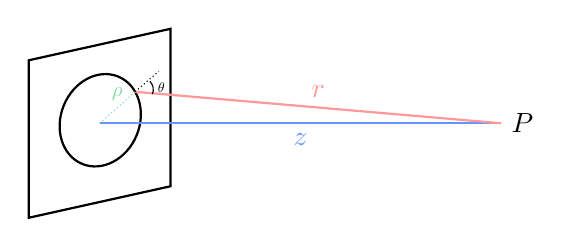
\begin{tikzpicture}
		\draw[thick] (-1,-1.2) -- (0.8,-0.8) -- (0.8,1.2) -- (-1,0.8) -- cycle;
		\draw[thick, rotate=-22.5] (-0.1,0) ellipse (0.5cm and 0.6cm);
		\draw[densely dotted,color=green!70!blue!50] (-0.1,0) -- (0.35,0.4) node[midway,above,scale=0.75] {$\rho$};
		\draw[thick,color=blue!70!cyan!60] (-0.1,0) -- (5,0) node[midway,below] {$z$} node [right]
			{\textcolor{black}{\( P \)}};
		\draw[thick,color=red!40!white] (0.35,0.4) -- (5,0) node[midway,above] {$r$};
		\draw[densely dotted] (0.35,0.4) -- (0.65,0.66);
		\draw (0.57,0.37) arc (-22.5:45:0.15cm) node[midway,right,scale=0.5] {$\theta$};
	\end{tikzpicture}
\end{center}

Assuming the point \( P \) is far enough away so that \( \theta \approx \frac{\pi}{2} \), then the \(
\mathbf{E}  \) field becomes:
\[
	\mathbf{E} = \frac{1}{4 \pi \epsilon_0 c^2}\frac{q \omega^2 x_0}{r} \cos\left[ \omega\left( t
	-\frac{r}{c} \right) \right]\hat{\boldsymbol{\theta}}
\]
Now to find the contribution due to the whole plane, we just integrate over the entire plane:
\[
	\mathbf{E} = \frac{1}{4\pi \epsilon_0 c^2}\int_\text{sheet} \frac{q \omega^2 x_0}{r}\Re\left[ e^{i \omega
	(t - r / c)} \right] 2 \pi \rho \eta \diff \rho
\]
Here, we define \( \eta \) to be the \textit{dipole density}, so the number of dipoles per unit area. We have
\( r^2 = \rho^2 + z^2 \), so \( r \diff r = \rho \diff \rho \), and hence:
\[
	\mathbf{E} = \frac{q \omega^2 x_0}{2 \epsilon_0 c^2}\int_z^{\infty} \Re\left[ e^{i \omega \left( t -
	\frac{r}{c} \right)} \right] \eta \diff r
\]
Now, if you assume that the sheet is uniform, then \( \eta = \eta_0 \), so we have:
\[
	\mathbf{E} = \frac{q \omega^2 x_0^2 \eta_0}{2 \epsilon_0c^2}\int_{z}^{\infty} \Re\left[ e^{i \omega
	\left( t - \frac{r}{c} \right)} \right] \diff r = \frac{q \omega x_0^2 \eta_0}{2 \epsilon_0 c^2}\Re\left[
\frac{c}{-i \omega} e^{ i \omega t} \left( e^{-i \omega (\infty) / c} - e^{-i \omega z / c} \right)\right]
\]
But the term in square brackets clearly diverges, so something has gone wrong here. In particular, it turns
out that our assumption that the dipole density is a constant, \( \eta = \eta_0 \), is not physical. So, we
need to "regularize" it by introducing a cutoff scale \( \Lambda \). We will do it as follows. Instead of
letting \( \eta(r) \) be a constant, we will instead define it as:
\[
	\eta(r) = \begin{cases}
		\eta_0 \left( 1 - \frac{r}{\Lambda} \right) & r < \Lambda\\
		0 & r > \Lambda
	\end{cases}
\]
It turns out that we not only need to regularize \( \eta \), but also do so in a way that is continuous. If
we were to just introduce an abrupt cutoff to \( \eta(r) \), then that discontinuity will also cause issues.
When we do this integral now, we will first assume \( \Lambda \) is finite, then take \( \Lambda \to \infty
\) after computing the integral. Now, using this refined \( \eta(r) \), we get the following result:
\begin{align*}
	\mathbf{E} &= \frac{q x_0 \omega^2 \eta_0}{2 \epsilon_0 c^2}\int_{z}^{\Lambda} 
	\Re\left[ e^{i \omega \left( t - \frac{r}{c} \right)}\left( 1 - \frac{r}{\Lambda} \right) \right] \diff r\\
			   &= \frac{\omega^2}{2 \epsilon_0 c^2} q x_0 \eta_0 \Re\left\{e^{i \omega t}\left[ 
					   {\color{blue!80!black}{\frac{c}{-i \omega}e^{i \omega \Lambda / c}}} - \frac{c}{-i
						   \omega} e^{-i \omega z / c} + 
						   {\color{blue!80!black}{\frac{c}{i \omega} e^{- i \omega \Lambda / c}}} 
						   - \frac{c}{i \omega}\frac{z}{\Lambda} e^{-i \omega z / c}
						   - \frac{c}{\omega^2} \frac{1}{ \Lambda} e^{-i \omega \Lambda / c} 
				   + \frac{c^2}{\omega^2}\frac{1}{\Lambda} e^{-i \omega z / c} 
		   \right] \right\} 
\end{align*}
Now, taking \( \Lambda \to \infty \), all \( \frac{1}{\Lambda} \) terms die off, and the two blue terms
cancel each other. So, we end up getting the result:
\[
	\mathbf{E} = \frac{\omega^2}{2 \epsilon_0 c^2}qx_0 \eta_0 \Re\left[ \frac{c}{i \omega} e^{i \omega \left(
	t - \frac{z}{c}\right)} \right] = \frac{\omega}{2 \epsilon_0 c}q x_0 \eta_0 \sin\left[ \omega\left( t -
\frac{z}{c} \right) \right]
\]
Then, remembering that \( x(t) = x_0 \cos(\omega t) \), then \( v(t) = -x_0 \omega \sin(\omega t) \), so:
\[
	\mathbf{E} = -\frac{q \eta_0}{2 \epsilon_0 c }v\left( t - \frac{r}{c} \right)
\]
And that's all we have for now. One thing you may have noticed in this integral is that the \( \Lambda \)
term didn't actually end up mattering -- we could have chosen the cutoff to be any number, and it would have
disappeared just the same. We will see why this is the case on Friday.    

 
  
